\documentclass{beamer}
\usepackage[utf8]{inputenc}
\usepackage[english]{babel}

% -- Including some standard packages --
\usepackage{graphicx}
\usepackage{soul}
\usepackage{hyperref}
\usepackage{colortbl}
\usepackage{dsfont}
\usepackage{soul}

% -- Choosing theme --

\usetheme{Boadilla}
\usecolortheme{whale}
% \usefonttheme[onlymath]{serif}

% Tikz
\usepackage{tikz}
\usetikzlibrary{matrix,positioning,fit,backgrounds,intersections}

% -- Cross signs --
\usepackage{pifont} % http://ctan.org/pkg/pifont
\newcommand{\cmark}{\ding{51}}%
\newcommand{\xmark}{\ding{55}}%
\newcommand{\xopt}{\ding{48}}%

% -- Custom commands --
\DeclareMathOperator*{\argmax}{arg\,max}
\DeclareMathOperator*{\argmin}{arg\,min}

\title[Mathematics I]{\textbf{Mathematics for Cryptographers. Preliminaries.}}
\author{ZKDL Camp}
\date{July 18, 2024}
\titlegraphic{
    
\includegraphics[width=0.2\textwidth]{images/logo.png}
}

\expandafter\def\expandafter\insertshorttitle\expandafter{%
  \insertshorttitle\hfill%
  \insertframenumber\,/\,\inserttotalframenumber}

\AtBeginSection[]{
  \begin{frame}
  \vfill
  \centering
  \begin{beamercolorbox}[sep=8pt,center,shadow=true,rounded=true]{title}
    \usebeamerfont{title}\insertsectionhead\par%
  \end{beamercolorbox}
  \vfill
  \end{frame}
}

\begin{document}
    \frame {
      \titlepage
    }
  
    \begin{frame}{Plan}
      \tableofcontents
    \end{frame}

    \section{Some words about the course}
    \begin{frame}{About ZKDL} 

      \begin{itemize}
        \item ZKDL Camp is a series of lectures and workshops on zero-knowledge proofs and cryptography.
        \item Here, we will learn state-of-the-art zero-knowledge systems: what are SNARKs, how they work under the hood from total scratch.
        \item Note, that this is not a regular course: we require a lot of commitment and the material is fairly complex.
        \item If possible, we will conduct workshops, where we will show practical implementations of the theoretical material.
      \end{itemize}

    \end{frame}

    \begin{frame}{Approximate Camp Structure}
      \begin{enumerate}
        \item Basic Mathematics: group and number theory, finite fields, polynomials, elliptic curves etc.
        \item Deep Delve into SNARKs: General definition, arithmetic circuits, commitment schemes, encryption etc.
        \item Analysis of modern zero-knowledge proving systems: Groth16, Plonk, BulletProofs, STARK etc.
        \item Specialization topics: low-level optimizations, advanced protocols such as folding schemes, Nova etc.
      \end{enumerate}
    \end{frame}

    \section{Number Theory}

    \section{Basic Group Theory}

    \begin{frame}{Why groups}

    \end{frame}

    \begin{frame}{Group Definition}
      \begin{definition}
        \textbf{Group}, denoted by $(\mathbb{G}, \oplus)$, is a set with a binary operation $\oplus$, obeying the following rules:
        \begin{enumerate}
            \item \textbf{Closure:} Binary operations always outputs an element from $\mathbb{G}$, that is $\forall a,b \in \mathbb{G}: a \oplus b \in \mathbb{G}$.
            \item \textbf{Associativity:} $\forall a,b,c \in \mathbb{G}: (a \oplus b)\oplus c = a \oplus (b \oplus c)$.
            \item \textbf{Identity element:} There exists a so-called identity element $e \in \mathbb{G}$ such that $\forall a \in \mathbb{G}: e \oplus a = a \oplus e = a$.
            \item \textbf{Inverse element:} $\forall a \in \mathbb{G} \; \exists b \in \mathbb{G}: a\oplus b = b \oplus a = e$. We commonly denote the inverse element as $(\ominus a)$.
        \end{enumerate}
    \end{definition}
    \end{frame}

    \begin{frame}{Group Examples}
      \begin{example}
        A group of integers with the regular addition $(\mathbb{Z},+)$ (also called the \textit{additive} group of integers) is a group. Indeed, an identity element is $e=0$, associativity obviously holds, and an inverse for each element $a \in \mathbb{Z}$ is $(\ominus a) := -a \in \mathbb{Z}$. 
      \end{example}
      
      \begin{example}
          The multiplicative group of positive real numbers $(\mathbb{R}_{> 0}, \cdot)$ is a group for similar reasons. An identity element is $e = 1$, while the inverse for $a \in \mathbb{R}_{>0}$ is defined as $\frac{1}{a}$.
      \end{example}
      
      \begin{example}
          The additive group of natural numbers $(\mathbb{N}, +)$ is not a group. Although operation of addition is closed, there is no identity element nor inverse element for, say, $2$ or $10$.
      \end{example}
    \end{frame}

    \begin{frame}{Explanation for Developers}
      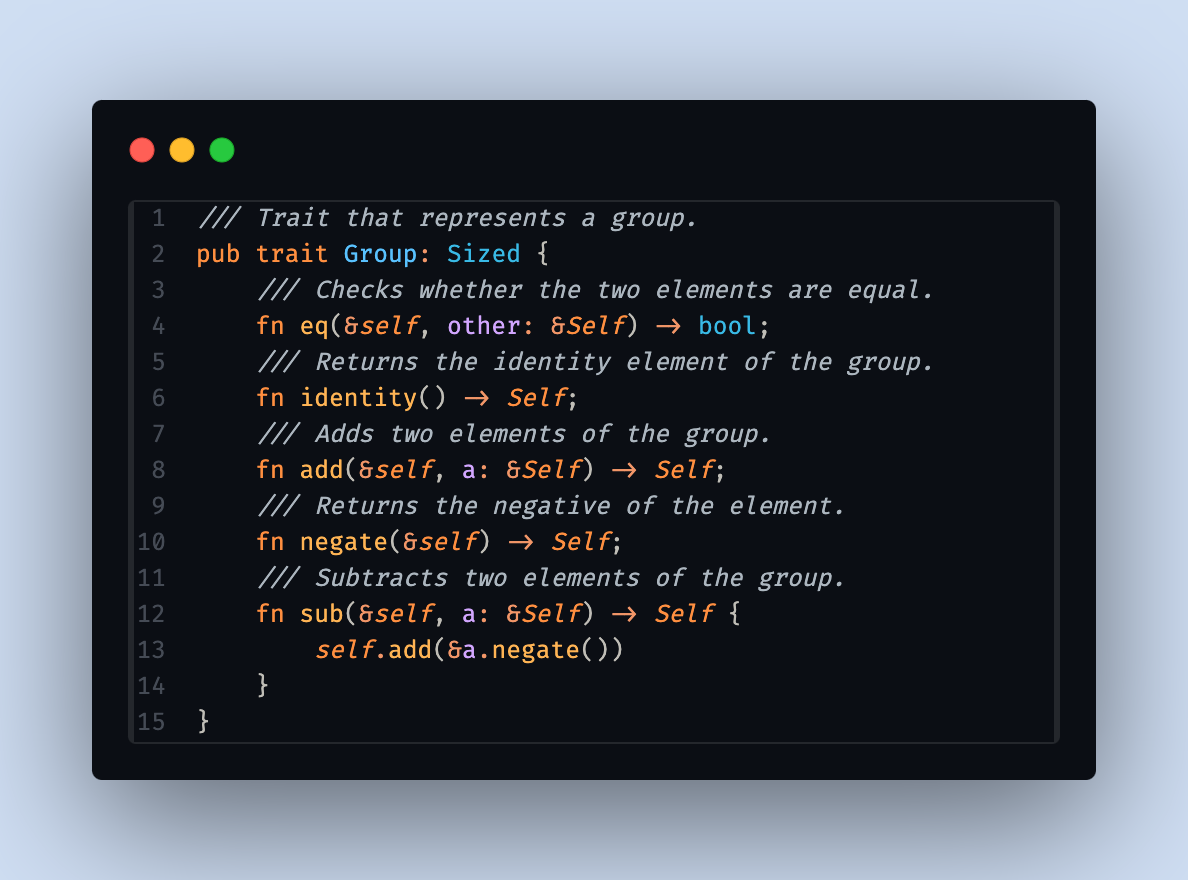
\includegraphics[width=\textwidth]{images/lecture_1/group_in_rust.png}
    \end{frame}

    \section{Polynomials}

      \begin{frame}{Field}
          \begin{definition}{}
              \textbf{Field} $K$ is a set equipped with appropriate \textbf{addition} and \textbf{multiplication} operations with the corresponding well-defined inverses, where you can perform the basic arithmetic.
          \end{definition}
          \pause
          \begin{exampleblock}{}
              \begin{itemize}
                  \item $\mathbb{R}$ (real numbers) is a field.
                  \item $\mathbb{Q}$ (rational numbers) is a field.
                  \item $\mathbb{C}$ (complex numbers) is a field.
                  \item $\mathbb{N}$ (natural numbers) is not a field: there is no additive inverse for $2$ ($-2$ is not in $\mathbb{N}$).
                  \item $\mathbb{Z}$ (integers) is not a field: additive inverse is defined, but the multiplicative is not ($2^{-1}$ is not defined).
              \end{itemize}
          \end{exampleblock}
      \end{frame}
  
    \begin{frame}{}
        \centering \Large
        \emph{Thanks for your attention!}
      \end{frame}
\end{document}